\documentclass{article}
\usepackage{xcolor}
\usepackage{graphicx}
\newcommand{\cliff}[1]{\ensuremath{C\ell\left(#1\right)}}
\newcommand{\ei}[1]{\ensuremath{{\bf e}_{#1}}}
\begin{document}

Manuscript Number: AACA-24-00133

\section*{Rebuttal to referees' comments}

Below, I reproduce the two reviews.  I have retrofitted the PDF to
\LaTeX, and made minor changes to the typesetting, but have not
changed the sense of the comments.  Replies to the issues, and my own
observations and general comments, are in \textcolor{blue}{blue}.  I
have indicated changes to the manuscript where appropriate.


\section*{Reviewer \#2}

\textcolor{blue}{ {\bf overall response to issues raised by reviewer
    \#2}.  Work of this type is always a balance between different
  audiences, and the reviewer seems to be pointing out that the
  submission lacks one or more aspects of work.}

  
\subsection*{0.1 Summary}

Referee recommends rejection of this paper which has been submitted for publication in AACA.
There are several reasons for this negative recommendation:
\begin{itemize}
  \item The mathematical content is nonexistent to the point that it
    appears that the Author has very little appreciation for
    mathematical structure of the (universal) Clifford algebra. In
    fact, the Author does not even give a definition of Clifford
    algebra or even give a reference to the definition that he uses.

\textcolor{blue}{Snygg was cited for its notation and Hestenes now
  cited.  I note that a definition of Clifford algebra was given in
  the original submission, albeit in a terse form.  Here I would point
  out that Clifford algebras do have a uniform definition across the
  references cited in the original submission and there is no genuine
  doubt as to the algebraic structure that I am considering.}

    The main objection is that the Author does not explain how he
    computes and encodes the algebra product which is critical to
    designing any package for computations with these algebras.

    \textcolor{blue}{I observe that the original manuscript included a
      substantial amount of high-level discussion of the codebase:
      ``The package represents basis blades using dynamic bitset
      objects\ldots''.  In any work of this type the author has to
      decide how much code to include in the manuscript.  On the one
      hand, readers of such a manuscript generally do not wish to be
      presented with a large amount of verbatim code; it is generally
      regarded as a featureless block of grey, of very little value [I
        edit two computational statistics journals and often instruct
        authors to remove code from their manuscripts; if I want to
        see code, I will look at it using a civilized coding tool, not
        browse a PDF].  Interested readers may consult the code
      directly (and here, as stated, the code is distributed under an
      open source license at github: the entire code base is open to
      inspection).\\[10pt] The other viewpoint---that of including
      substantial extracts from the codebase---is being espoused by
      the referee.  There are occasions where this approach is
      justified, but I do not agree that this is one of them.  The
      following figure shows what is in many ways the core of the C
      backend of the associated software, in this case the direct
      definition of six of the definitions of ``multiplication''
      implemented in the package:\\[10pt]
      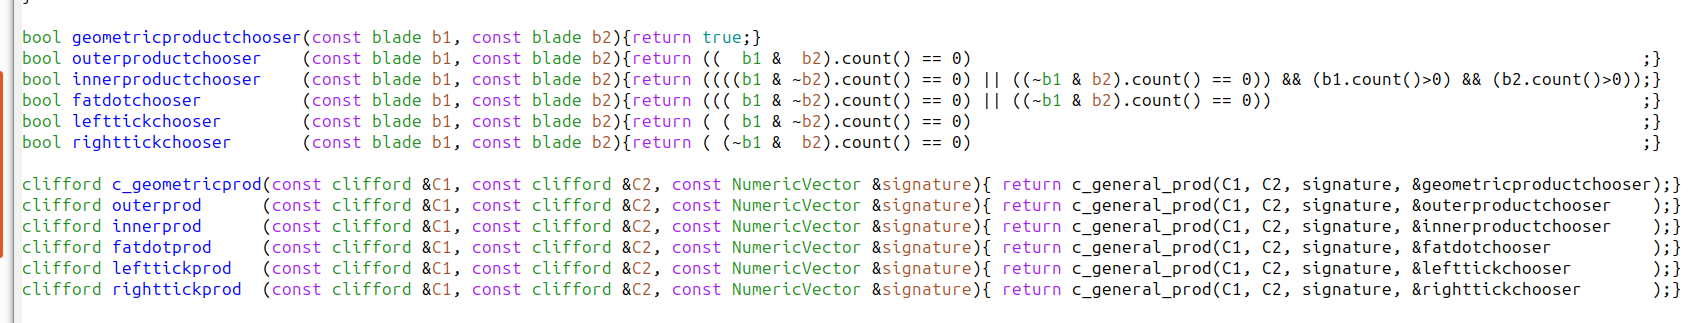
\includegraphics[width=6in]{code.png}\\[10pt] Surely the referee
      is not suggesting I include such material in the manuscript?
      Nevertheless, on reflection, the submission does not reflect the
      large codebase present in the R package, and I have added
      pointers to the github account so interested readers can inspect
      the code in a suitable interactive environment.}
      
    In particular, from the text in Section 7 it appears that the
    Author uses identities (7.1) and (7.2) as his/her definitions of
    the contractions, which is mathematically wrong\footnote{By the
    way, the Author does not explain the syntax of such input anyway}

    \textcolor{blue}{The definitions are lifted from Dorst 2002 which
      was not cited explicitly in the manuscript.}

    \ldots whereas the left contraction (and similarly the
    right contraction) has been defined independently of the Clifford
    product (cf. [6, Sections 22.1 and 22.2]). Then, the left
    contraction is used, following the well-known Chevalley’s
    construction, to define the Clifford product via the formula

    $$
    \mathbf{x}u=\mathbf{x}\wedge u + \mathbf{x}\rfloor u,\qquad\mathbf{x}\in V,u\in\bigwedge V
    $$

and then extended by linearity and associativity to all of V [6, Page
  290] which yields an algebra isomorphic to the Clifford algebra
\cliff{Q} (or, \cliff{p, q, r})\footnote{It is strange that the Author
does not even explain the relation between a quadratic space (V, Q)
and the (universal) Clifford algebra \cliff{V, Q}, also denoted in the
literature as \cliff{Q} cf. [6].

\textcolor{blue}{Explaining the relation between $(V,Q)$ and the
  universal Clifford algebra would not add any value to a manuscript
  discussing a computational implementation.  The manuscript was
  prepared to appeal to a particular level of abstraction and
  discussion of category-theoretic characterisation of Clifford
  algebras is clearly not in scope.}  } \footnote{In fact, the
Chevalley’s construction works for a Clifford algebra \cliff{B} of any
bilinear form B and an extensive package already exists for
computations with these algebras [1, 2].

\textcolor{blue}{The reviewer states a true fact, one that would not
  add any value to a manuscript discussing a computational
  implementation.}} \footnote{Observe that when the Clifford product
xu is defined as in (1), which amounts to V defining the Clifford
algebra \cliff{Q} as a subalgebra of the algebra of endomorphisms of
the Grassmann algebra V, it is necessary to encode in any package
(based on this definition) both the Clifford product and the Grassmann
product. However, in the package clifford of the Author, there is no
provision for computing the wedge product

\textcolor{blue}{This statement is simply false.  A cursory inspection
  of the package reveals that the wedge product is implemented as an
  overloaded caret (``{\tt\string^}'').  This device is documented
  according to standard documentation protocols and is apparent on
  viewing the default landing page for the package manual, and indeed
  on the pkgdown website.  I cannot see how one could make the wedge
  product more visible to users.}  }

\textcolor{blue}{The above comments are true, but I do not see any
  constructive comments here.  The identity $\mathbf{x}u +
  \mathbf{x}\wedge u+\mathbf{x}\rfloor u$ is true, as demonstrated
  in the following R session:\\[20pt]
{\tt > x <- rcliff(d=5)}\\
{\tt > u <- as.1vector(sample(1:10,5))}\\
{\tt > }\\
{\tt > x}\\
{\tt Element of a Clifford algebra, eual to}\\
{\tt + 7 + 8e\_2 - 9e\_3 - 1e\_13 - 2e\_4 - 5e\_234 + 9e\_5 - 8e\_25 + 6e\_1235 - 4e\_2345}\\
{\tt > u}\\
{\tt Element of a Clifford algebra, equal to}\\
{\tt + 10e\_1 + 9e\_2 + 3e\_3 + 2e\_4 + 4e\_5}\\
{\tt > x*u == x\string^u + x\%|\_\%u}\\
{\tt [1] TRUE}\\
{\tt > }\\
}

Thus, it is a
serious deficiency not to explain how the Clifford product and the
contractions are defined and computed in the package.  Of course,
there are other ways to compute the Clifford product and especially in
the algebras $\cliff{p, q} = \cliff{p, q, 0}$ generated by an
orthonormal basis such as the one based on Walsh functions cf. [6,
  Chapter 21]. The algorithm presented in [6, Section 21.3] applies to
the Clifford algebras \cliff{p, q} but it has been expanded in [3] to
include the degenerate quadratic forms for the algebras $\cliff{p, q,
  r}, r > 0$.

\textcolor{blue}{The referee observes an interesting part of a
  textbook.  I do not understand in what way this comment can be
  construed as a constructive comment.}

Nevertheless, the Author does not provide any hint
which algorithm he has used in his package.

\textcolor{blue}{That is not true.  The original submission included a
  discussion of how [boost C++ library] bitsets are used in the
  implementation; the actual code used for Clifford is a
  straightforward application.  Admittedly, bitsets are a somewhat
  specialized and arcane aspect of the boost program, and I have
  arguably assumed knowledge of them that might not be familiar to
  ACAA readership.  On reflection more detail might have been
  appropriate.  So, I have added a brief explanatory note (in
  \textcolor{blue}{blue}) to the manuscript.}

\item According to Wikipedia [7], “R is a programming language for statistical computing and
data visualization. It has been adopted in the fields of data mining, bioinformatics, and data
analysis.” and “Packages add the capability to implement various statistical techniques such
as linear, generalized linear and nonlinear modeling, classical statistical tests, spatial analysis,
time-series analysis, and clustering.”
Thus, it is really puzzling why the Author has selected the R language as the programming
language for his/her package: it should be clear from this manuscript, that this language is
highly unsuitable for such task.

\textcolor{blue}{The project gives R users transparent access to
  Clifford algebra.  As the manuscript demonstrates, the R language is
  not ``highly unsuitable'' for this task.  Certainly, it is not
  straightforward, but the resulting package furnishes Clifford
  algebra constructs in an R-centric manner.  The package now allows
  seamless R idiom to work with Clifford algebra simultaneously with
  the considerable codebase [over 20000 packages and counting].}

For one, the language is meant to deal with commuting numerical
input. As a consequence, the Author uses the same symbol $*$ for the
scalar product as in $5* e(1)$ and in $x * x$ (see page 1 and later)
where $x$ is an element in a Clifford algebra.  Thus, the Author
ignores the fact that the Clifford product is non-commutative in
general, and so another symbol should be used for it in the package.

\textcolor{blue}{I am not ``ignoring the fact that the Clifford
  product is non-commutative''.  Cursory inspection of the package
  would show that the entire codebase is predicated on the
  noncommutative nature of the geometric product.  It would be more
  appropriate (and more constructive) to view the package as providing
  natural R idiom for working with Clifford algebra.  The reviewer
  appears to be unaware of the standard concept of ``overloading'' in
  C++ and indeed R.  Briefly, overloading in C++ is compile-time
  polymorphism, and in R is run-time polymorphism.  In the package
  this standard concept is applied, {\em inter alia}, to the $*$
  operator.  When parsing an expression such as {\tt a*b}, R
  dispatches to a binary operator that depends on the classes of {\tt
    a} and {\tt b}.  Now, if object {\tt a} happens to be a scalar,
  then an appropriate scalar product operator is called.  If both {\tt
    a} and {\tt b} are Clifford objects, the geometric product
  operator is called.  The object-oriented nature of R can easily cope
  with these distinctions, and I leverage the S3 and S4 mechanisms to
  accomplish these operations using natural R idiom.}

For two, the syntax of the R language does not support standard
mathematical notation because it explicitly outputs terms like

\begin{verbatim}
  + 8 + 1e 1 - 10 e 2 -1e 12 ...
\end{verbatim}

instead of just

\begin{verbatim}
  8 + e 1 - 10e 2 - e 12 ...
\end{verbatim}

\textcolor{blue}{This is not a feature of the syntax of the R
  language.  It is a feature of the print method.  R packages
  generally include bespoke methods to display R objects using S3 or
  S4 dispatch.  Perhaps the reviewer was unaware of this.  Is the
  reviewer {\em really} commenting on the presence of a plus sign at
  the beginning of a line of output, interpreting it as R ``not
  supporting standard mathematical notation''?.  The presence of the
  plus sign was a deliberate and conscious design decision.  It
  ensures consistency and allows for easy parsing of output.  R is
  sufficiently flexible to change it [a one-line modification of
    function {\tt print\_clifford\_default()} would suffice], but the
  form was chosen with care and should not be changed.}

(see page 3 and later). Furthermore, the input is extremely awkward
like, for example,

\begin{verbatim}
  x <- clifford(list(1:3),c(2,3,7)),coeffs=3:4)
\end{verbatim}

on page 5 or

\begin{verbatim}
  (x <- clifford(list(1:3,c(1,5,7,8,10)),c(4,-10)) + 2)
\end{verbatim}

 on
page 7\footnote{By the way, the Author does not explain the syntax of
such input anyway.}

\textcolor{blue}{One goal of the submission was to introduce a variety
  of different package constructs, including methods that might appear
  overly rigid.  Given this, it is perfectly sensible to include an
  example of function {\tt clifford()}, the formal creation method
  used in the package.\\[10pt] If one is not familiar with good
  practice in object-oriented languages such as R or C, idiom such as
  reproduced above by the reviewer might appear unnatural or awkward.
  However, careful reading of the manuscript reveals that this
  particular syntax is the {\em formal} creation method.  Along with
  operator overloading, this is a commonly-used feature of C++ and R.
  Such constructions are included in many introductory texts,
  including those cited in the submission.  Nevertheless, as the
  reviewer implies, it is possible that some readers will have little
  experience with standard techniques such as this, and to these
  readers such constructions might appear difficult or unnecessarily
  rigid.  I have added a brief explanation that might dispel any
  confusion.}

\item The Author does not distinguish the unity 1 of the real field R
  from the Clifford algebra unit element. Let us denote the algebra
  unit by say $\mathbf{1}$. While we often write $1 + e_1 + 2e_{23}$
  and we do identify the number 1 with the term $\mathbf{1}$ in the
  algebra (due to the isomorphism $k\longrightarrow k\mathbf{1}$ where
  $k$ is a field) we cannot treat 1 as the scalar scalar (1) equal to
  \verb+e(2)*e(2)+ as shown on page 4 because that product really
  equals $\mathbf{1}$.  While this may appear as a minor issue when
  writing a paper, it shows a shortcoming of the package, probably
  caused by the very limited ability of the R language to deal with
  symbolic input and output, and hence inability to distinguish
  between 1 and 1.

  \textcolor{blue}{As stated above, these concerns are immaterial if
    one is familiar with the elementary concept of overloading of
    operators.  I am having difficulty interpreting the reviewer's
    comments as informed constructive criticism.  Phrases such as
    ``limited ability of the R language'' [which are demonstrably
      incorrect] do not help.  The R language has extensive
    documentation which includes extensive coverage of this issue, and
    the standard reference is cited in the submission.}

  Yet, when designing any package for Clifford/Grassmann algebras,
  such distinction is crucial.

  \textcolor{blue}{The distinction is not necessary if one has
    operator overloading at one's disposal.  While I appreciate that
    some segments of ACAA readership might not be familiar with
    overloading, I feel that there are better ways to introduce the
    concept than including a ``how to use overloading in R'' in the
    submission.}
  
\item On page 6 in Section 6 Author computes the product $e(53)^2$ in
  a Clifford algebra of a positivedefinite inner product. The answer
  given by his/her package as \verb+scalar( 1 )+ is clearly wrong
  since, using his/her notation,

  $$
  e(53)^2=e(5)*e(3)*e(5)*e(3)=-(e(5)*e(5))*(e(3)*e(3))=-1
  $$

given that $e(5)*e(5)=e(3)*e(3)=1$ and $e(5)*e(3)=-e(3)*e(5)$.  Thus,
the question arises whether the Author’s algorithm for computing the
Clifford product miscomputes, although other products computed in the
paper, e.g., $x * x$ and $y * x$, are correct, or, perhaps there is a
typo in that paragraph on page 6.  Since the Author does not explain
his/her algorithm, nor he provides the code for his/her procedure $*$
referee cannot trace the source of this error\footnote{Author does not
explain how the compiler distinguishes between the symbol $*$ used as
the Clifford product as in $x * x$ and the same symbol $*$ used as a
scalar product as in $2 * e(2)$.

\textcolor{blue}{Again, the {\tt *} symbol is overloaded.  A
  description of the concept of overloading would be superfluous for
  the intended readership.}  }

\textcolor{blue}{This issue was caused by a misreading of the
  manuscript, which says, as intended that $(e_{(53)})^2=1$ (that is,
  element number fifty three squared).}

\item The package clifford presented in the paper is extremely
  limited. It only has a few functionalities such as the computation
  of the Clifford product $*$; addition/subtraction in the algebra; a
  random generation of Clifford algebra elements by a procedure
  \verb+rcliff+ although its syntax is not explained;
  \textcolor{blue}{Brief explanation now included} the left and the
  right contractions although it is not clear how they are computed;
  probably there is a procedure for computing the r-vectorpart
  $\left\langle A\right\rangle_r$ of a general Clifford algebra
  element A\footnote{ Author does not explain the notation
  $\left\langle A\right\rangle_r$

  \textcolor{blue}{The grade notation $\left\langle A\right\rangle_r$
    is standard.  See, for example, Hestenes or indeed Snygg, both
    standard reference texts.  I have cited the notation for the
    benefit of those unfamiliar with these textbooks.}}
  The package
  has none of the three main automorphisms built-in such grade
  involution; reversion; and conjugation [6] which is a must-to-have
  in any package.

\textcolor{blue}{These comments are demonstrably false.  The
  manuscript presented a small subset of the capabilities of the
  package.  A cursory inspection of the package would reveal the rich
  structure of the package.  For example, as enumerated in the
  documentation, there are five different types of multiplication, and
  six different types of conjugation.}
  
\item The paper, whose purpose is to present Author’s package clifford, is very awkwardly written
since:

\begin{itemize}
\item no code is given of any procedure;

  \textcolor{blue}{As stated above, snippets of the C++ back-end would
    be inadvisable in the manuscript, and the code is readily
    inspectable on github}
\item  no mathematics behind any procedure is provided;

  \textcolor{blue}{More detail is given in the introduction}
\item no comparison is made between this very simple package with any of the existing packages;

  \textcolor{blue}{No R functionality for Clifford algebra is available}

\item  no summary of the package functionalities is given;

    \textcolor{blue}{Table of products and conjugations now included}

\item  no explanation or reason is given by the Author why he/she is attempting to write yet
a new package for Clifford/Grassmann algebras in this very limiting non-symbolic R
programming language given that many other much more comprehensive packages for
Clifford/Grassmann algebras exist including a very fast package called eClifford for
the Clifford algebras C`(p, q, r). See, for example, [1, 2, 3].

\textcolor{blue}{Firstly, I must take issue with the somewhat weighted
  phrase ``very limiting non-symbolic R programming language''.  There
  are a wide range of symbolic packages available in the R language.
  I would include native R capabilities for Weyl algebra, multivariate
  polynomials, graph theory, finite group theory, and many many
  others.  I have cited some of the more prominent examples.  It is
  simply incorrect to characterise R as a non-symbolic language.}

  \textcolor{blue}{Secondly, the Maple language is propietary.  One
    benefit of the R language is that it is open-source.  Maple
    libraries might exist but the language is not open-source, which
    disbars it for many people.  But, noting that these citations are
    behind a paywall, I do cite the referee's citations in the
    manuscript.  Although they do claim to be ``available from R'',
    such functionality is typically somewhat poorly linked to the
    wider R codebase.  For example, it is difficult to manipulate the
    objects using natural R idiom, and difficult to extract
    information to pass to other parts of the wider R ecology.
    Similar systems also ``available from R'' in the open-source world
    might include interfaces to sage, maxima, gap, etc.  These
    uniformly do not include a natural interface that allows one to
    exploit the many features of the R language.
 }

\end{itemize}

\item AACA “publishes high-quality peer-reviewed research papers as well as expository and survey
articles in the area of Clifford algebras and their applications to other branches of mathematics,
physics, engineering, and related fields.” [5]. Unfortunately, the submitted manuscript is too short,
it is not well written, and it does not report on any significant development and that includes the
program clifford which is, at best, in its early stages of development. However, the R language,
in the opinion of this reviewer, is not suitable for developing a package for Clifford algebras for the
reasons summarized above.

\textcolor{blue}{The R language is evidently suitable for developing a
  package for the Clifford algebra.}

\end{itemize}

\subsection*{0.2 Detailed comments}

In the following, referee provides some additional comments on the text.

\begin{enumerate}
  \item Abstract: This fragment “a range of different multiplication operators is provided” is confusing since only one multiplication in the Clifford algebra is provided (although not defined),
    namely, the Clifford product $*$.

    \textcolor{blue}{As discussed above, this comment is factually
      incorrect. I have included a table showing the most common
      multiplications and the most common convolutions.    }

    
\item Page 2: The last two paragraphs in Section 1 are confusing.
  Namely, we want the vectors $e_1,\ldots e_n$ to provide a basis in
  an $n$-dimensional real vector space $V$ rather than just span the
  space.  Then, we know that the (universal) Clifford algebra
  \cliff{V} is finite-dimensional of dimension $2^n$

  For the basis vectors $e_i , i = 1, \ldots n$, to anti-commute in
  \cliff{V}, that is, $e_i e_j = -e_i e_j$ for $i\neq j$, we must
  require that the basis vectors are orthogonal.  Furthermore, $p + q$
  such vectors are in fact orthonormal which, in the algebra
  \cliff{V}, satisfy $e_i^2 = 1$ for $1\leq i\leq p$ and $e_i^2 = -1$
  for $p+1\leq i\leq p+q$ while $e_i^2 = 0$ for $p + q + 1 \leq i\leq
  n$.  Let $r=n-p-q$.  Thus, on the $(p + q)$-dimensional subspace W
  of V with a basis $e_i, 1\leq i \leq p+q$ we have a non-degenerate
  quadratic form Q of signature ($p, q)$ while on its orthogonal
  complement $W^\bot$ of dimension r we have a null quadratic form
  Q0. Thus, in short, in display (1.1) instead of “otherwise” we
  should have this range $p + q + 1 \leq i \leq n$.  Then, such
  Clifford algebra \cliff{W\bot W^\bot} is denoted as \cliff{p,q,r}
  rather than \cliff{p,q}. In the special case when $p = q = 0$, we
  have $\cliff{0,0,r}\simeq\bigwedge V$ or $C\ell_{0,0r})$ where
  $\bigwedge V$ is the Grassmann algebra.
  \textcolor{blue}{This is actually a reasonable comment.  Corrected.}
  
\item  Page 2 Section 2: Author does not
  explain what a “blade” is.
  \textcolor{blue}{Standard definition of blade now included.}
  \item Page 2: display at the bottom of the
page: This display has absolutely no meaning to the reader because the
Author does not explain what it means.

\textcolor{blue}{On the one hand, the referee complains that I do not
  explain how I compute the products, yet when I do include
  informative code extracts, the referee complains that he does not
  understand it.  Anyone familiar with C++ would be able to interpret
  these lines and understand that the computational back-end operates
  on STL map classes with boost bitsets as keys and (IEEE) real
  numbers as values.}

\item Page 3: This sentence “This
is not an issue for the maps considered here as addition and
multiplication are commutative and associative.” is puzzling since the
Clifford product is non-commutative for $n > 1$.

\textcolor{blue}{This was an error, the word ``multiplication'' should
  not have been there, now removed.}

\item Pages 2, 3, and
later: Referee has already commented on the very awkward (and
practically unusable) input/output of the R language.

\textcolor{blue}{Just to be absolutely explicit here, the {\tt
    clifford()} function is the formal creation method but, as
  explained at length in the submission, day-to-day package idiom
  includes much nicer and more convenient idiom for creating clifford
  objects, for example\\[20pt]
{\tt
> 6 - 4*e(3) +11*e(1:4)\\
Element of a Clifford algebra, equal to\\
+ 6 - 4e\_3 + 11e\_1234\\
> \\
}
I don't see any awkwardness or infelicity in this creation method.}
  

\item Page 3:
nowhere on page 3 the reader is informed what signature has been used
to compute the products $x * x$ and $z * x$. Only later on page 4 the
reader finds out that the default is the signature (p, 0, 0).

\textcolor{blue}{Corrected.}

\item Page 4: the last display in Section 3 has absolutely no meaning to the
  reader because the Author does not explain what it means.

  \textcolor{blue}{{\tt disordR} compliance was discussed in the
    previous section of the original submission.  However, on
    reflection, I now think the issue of {\tt disordR} discipline is
    likely to be a distraction for likely ACAA readership and on
    balance I think it might be better to give the grades of the
    result in standard R vector format.  In any event, I have added a
    short discussion of the {\tt disordR} package (and cited the
    canonical reference to it).  I have also changed the presentation
    of the output that the reviewer queries to use standard R vector
    output, so it does not include the hash code and comment about the
    order of the elements (which I now feel was a unnecessary
    distraction).}

\item Page 4: what is the meaning of
  $n=\left[\begin{array}{cc}1&0\\0&-1\end{array}\right]$ when $n$ was
  defined as a positive integer on page 2?  \textcolor{blue}{This is
    an alternative notation for the signature that the reviewer points
    out has not been introduced.  I have rewritten in $(p,q)$
    notation.}
  
  \item Page 5: the display after the words
“then the stokes idiom for this would be: ...” has absolutely no
meaning to the reader because the Author does not explain what it
means.

\textcolor{blue}{I note that the original manuscript introduced and
  cited the {\tt stokes} package in the previous paragraph.  On
  reflection the text is perfectly clear if one can hold the content
  of the previous paragraph in one's mind.}

\item Page 6: it was already remarked above that in signature $(p, 0,
  0), p > 0$, the square of $e_{53}$ is -1 and not 1 as shown in the
  output \verb+scalar ( 1 )+.

\textcolor{blue}{Discussed above, the reviewer misread the
  manuscript.}

  \item Page 6: Formulas (7.1) and (7.2) are not stated correctly: we
    must require $s\geq r$ in (7.1) and $r \geq s$ in (7.2) with
    additional statements that $\left\langle
    A\right\rangle_r\rfloor\left\langle B\right\rangle_s=0$ and
    $\left\langle A\right\rangle_r\lfloor\left\langle
    B\right\rangle_s=0$ when $s > r$.  Thus, in the double summation
    in (7.1), the term $\left\langle\left\langle
    A\right\rangle_r\left\langle B\right\rangle_s\right\rangle_{s-r}$
    must be replaced with 0 when $r > s$ and in the the double
    summation in (7.2), the term $\left\langle\left\langle
    A\right\rangle_r\left\langle B\right\rangle_s\right\rangle_{r-s}$
    must be replaced with 0 when $s>r$. Apparently, these two special
    cases have been correctly encoded because the two examples for
    $A\rfloor B$ $A\lfloor B$ have correct outputs.\footnote{The referee notes that the Author does not explain the
meaning of this notation: $\left\langle A\right\rangle_r$.}
\footnote{The referee also notes the awkwardness of this syntax {\tt
  \%\_|\%} for the left contraction and {\tt \%|\_\%} for the right
contraction in clifford.\textcolor{blue}{ The issue of ``awkwardness''
  is discussed above.}}

\textcolor{blue}{First, I note that these two operations are in fact
  correctly implemented, as the referee indicates.  The equations are
  drawn verbatim from Dorst (2002), who saw no need to add a
  superfluous indicators such as $s>r$. This would be understood by
  most readers.  As regards the ``awkwardness'' of these notations,
  the package also allows functional notation: {\tt x\%|\_\% y} {\tt
    x\%\_|\% y} may be evaluated using {\tt lefttick(x,y)} and {\tt
    righttick(x,y)} respectively, as detailed in the list now included
  in the appendix.}

\item Page 6: the comment at the bottom of page 6 which extends to the
  end of Section 7 on page 7 above Section 7.1, points to an
  irrelevant and awkward peculiarity of the R language and it does not
  deserve to be a part of the text: a footnote would suffice
  explaining why there is a need for the extra parentheses when
  computing $e_2\rfloor (e_1e_2)$.

  \textcolor{blue}{This is not an ``awkward and irrelevant
    peculiarity'', this is ``a result of a well-considered parsing
    mechanism that might be confusing to users of the package''.  This
    particular language feature caught me out more than once and I
    feel that including a brief sentence or two outlining the issue is
    beneficial.}

    
\item Page 8: he conclusions and further work statements are
  insufficient in view of many functionalities that are still missing
  in clifford including the lack (already mentioned) of the three
  automorphims. \textcolor{blue}{As discussed above, the package
    includes a number of automorphisms, now detailed in an appendix.}
  It should also be pointed out that the Author does not mention any
  ability on the part of the R language for handling matrices, let
  alone symbolic matrices.  Thus, it is not known whether it would be
  even possible to handle spinor or regular representations of the
  Clifford algebras \cliff{p, q, 0} in clifford.
  \textcolor{blue}{Casual familiarity with the R language would reveal
    extensive R capability for handling matrices.  There is a certain
    amount of functionality for symbolic matrix manipulation.  I have
    added a citation to two such journal articles [for dealing with
      octonionic matrices or Jordan algebra].}  Finally, the author
  does not explain what the stokes package is and why he would want to
  \ldots{\em include closer integration with the stokes package}\ldots

  \textcolor{blue}{I note that the {\tt stokes} package was cited in
    the original submission.  However, in the time between submission
    and now, I now believe that both the {\tt stokes} package and the
    {\tt clifford} package are sufficiently self-contained for closer
    integration not to be sensible idea.}


\end{enumerate}

\section*{References}

\begin{description}
\item{[1]} R. Ablamowicz and B. Fauser: Mathematics of CLIFFORD: A Maple Package for Clifford and
Grassmann Algebras, Adv. Applied Clifford Algebras 15 (2) (2005), 157–181.\\
\item{[2]} R. Ablamowicz and B. Fauser: CLIFFORD: A Maple Package for Clifford and Grassmann
Algebras for Maple 2020, available from R. Ablamowicz at {\tt rablamowicz@gmail.com}, 2024.\\
\item{[3]} R. Ablamowicz: eCLIFFORD: A Maple Package for Clifford and Grassmann Algebras \cliff{p, q, r}
for Maple 2020, available from R. Ablamowicz at {\tt rablamowicz@gmail.com}, 2024.\\
\item{[4]} Maple 2020.2, November 11, 2020, Copyright Maplesoft, a division of Waterloo Maple Inc.
1981-2020.\\
\item{[5]} Advances in Applied Clifford Algebras, Aims and Scope,
{\tt https://link.springer.com/journal/6}, August 2024.\\
\item{[6]} Lounesto, P., Clifford Algebras and Spinors, 2nd. ed., Cambridge University Press, 2001.
\item{[7]} R (programming language) Wikipedia, The Free Encyclopedia,
{\tt https://en.wikipedia.org/wiki/R (programming language)}, August 2024.
\end{description}


\section*{Reviewer \#3}

\textcolor{blue}{Overall response to reviewer \#3: I am delighted that
  this insightful referee ``gets'' the package.  They make some
  comments which I respond to below.}


The paper introduces a new R package for Clifford algebra. The package
uses a sparse representation for both basis blades and multivectors
for efficiency of representation.  Arbitrary signatures for the basis
vectors can be defined by the user.

\textcolor{blue}{Yes! the characterisation as ``sparse'' is insightful
  indeed: the efficiency of the bitset class was a major driver behind
  the back-end architecture of the package.}

On the positive side, R is an important computational environment for
statistical computing and data science, the introduction of Clifford
algebra to R is a welcome and appreciated effort.

Unfortunately, I have to recommend the author make some important
major changes in the paper to be accepted for publication due to the
following points:

\begin{itemize}
  \item Are there any other R packages for Clifford algebra? This
    should be explicitly stated in the paper.
  \item The paper has no mention of how the main products (geometric,
    outer, left/right contraction) are actually implemented on
    multivectors. This is a significant computational bottleneck in
    similar libraries.

\item How is this package useful when we have many multivectors
  (hundreds or thousands) to work with? After all, R is mainly used
  for statistical and data science computations and a use-case where
  only a few multivectors are used is not so useful in this context.
\item The paper also lacks comparison with other similar packages in
  terms of (for example): performance, memory requirements, design
  goals, possible use cases, integration with R statistical
  computation capabilities, implemented algebraic operations on
  multivectors, support for outermorphisms, etc.
\item Some other points include: Page 3: The notation for a Clifford
  Algebra should be modified to become $\cliff{p,q,n-p-q}$ with $p\geq
  0$, $q\geq 0$, $p+q\leq n$.
\textcolor{blue}{This is a reasonable point, but I must respectfully
  disagree.  The package's primary contribution is that of R-centric
  functionality.  In the R world, the word ``vector'' refers to a
  basic data structure that represents a one-dimensional array of
  (real) numbers.  The key fact is that the length of a vector is not
  specified until it is created.  In R, then, one way of working is to
  define a vector that is long enough so that one can manipulate the
  first few elements, and forget about its exact length.  For example,
  we might define a vector of zeros with length 6:\\[20pt]
  {\tt > x <- rep(0,6)   \# repeat "0" six times and assign to x, a vector}\\
  {\tt > x\ \ \ \ \ \ \ \ \ \ \ \ \ \# what is x?}\\  
  {\tt [1] 0 0 0 0 0 0\ \# x is just six zeros}\\
  {\tt > x[3] <- 1\ \ \ \ \ \# assign "1" to element 3 of x}\\
  {\tt > x\ \ \ \ \ \ \ \ \ \ \ \ \ \# what is x?}\\  
  {\tt [1] 0 0 1 0 0 0\ \# element 3 of x updated to 1}\\[20pt]
Above, when using {\tt x[3] <- 1}, one does not care what the length
of the vector x actually is, so long as it is greater than or equal to
3.  It is very convenient to forget that {\tt x} is actually of length
6. This kind of thinking is pervasive in the R world.  This is
compellingly similar to the world of Clifford algebra, where one does
not really need to know the dimensionality of the underlying vector
space $V$, so long as it is ``big enough''.  Specifically, if one is
working in $\cliff{p,q}$, one can assume that $n\geq p+q$ where
$n=\dim(V)$.  If this is so, it is natural to forget the exact value of
$n$, on the grounds that \ei{i}\ei{i}=0 for any $n\geq p+q$.\\[10pt]
However, sometimes one needs to explicitly respect the value of $n$
and the package has a mechanism [option {\tt maxdim}] to enforce this
if needed.  This issue is not super-important in daily use [the docs
  state that {\tt maxdim} is a ``super-strict safety measure''] and I
have added a brief discussion to a footnote in the manuscript.  }

\item Page 4: I'm not sure what {\tt rcliff()} function does, is it a
  random multivector generator? If so, why are all scalar coefficients
  integers?

  \textcolor{blue}{Function {\tt rcliff()} does indeed return a random
    element of a Clifford algebra.  The coefficients are integers in
    order to give an object with a compact representation.  The
    function uses random sampling from small integers to generate the
    coefficients.}

\item Page 5: What does the {\tt include.fewer=TRUE} flag serve?

  \textcolor{blue}{The {\tt include.fewer} flag takes a logical
    argument with {\tt FALSE} meaning to return a clifford object all
    of whose terms are the specified grade, and {\tt FALSE} meaning to
    include terms with grades less than the specified grade.  I have
    included [on page 4] a brief explanation on the manuscript.}
    
\item Page 6: Does ``{\tt x \%\string^\% y}'' mean the outer product
  operation?  Please clarify the correspondance of R operators to
  Clifford algebra operations in a small table in the paper.

  \textcolor{blue}{It is a wedge product as detailed in the new table
    in appendix A}

\end{itemize}

\end{document}
